%----------------------------------------------------------------------------------------
%	PACKAGES AND DOCUMENT CONFIGURATIONS
%----------------------------------------------------------------------------------------

\documentclass{article}

\usepackage[version=3]{mhchem} % Package for chemical equation typesetting
\usepackage{siunitx} % Provides the \SI{}{} and \si{} command for typesetting SI units
\usepackage{graphicx} % Required for the inclusion of images
\usepackage{natbib} % Required to change bibliography style to APA
\usepackage{amsmath} % Required for some math elements 
\usepackage{placeins}
\usepackage[font=small,labelsep=space]{caption}
\captionsetup{%
  figurename=Fig.,
  tablename=Table
}
\setcitestyle{square}
\setlength\parindent{0pt} % Removes all indentation from paragraphs

\renewcommand{\eqref}[1]{\textup{{\normalfont(\ref{#1}}\normalfont)}}

\renewcommand{\labelenumi}{\alph{enumi}.} % Make numbering in the enumerate environment by letter rather than number (e.g. section 6)

%\usepackage{times} % Uncomment to use the Times New Roman font

\textheight=8.5in
\topmargin=-0.5in

%----------------------------------------------------------------------------------------
%	DOCUMENT INFORMATION
%----------------------------------------------------------------------------------------

\title{Homework 1} % Title

\author{Kenneth \textsc{Chaney}} % Author name

\date{\today} % Date for the report

\begin{document}

\maketitle % Insert the title, author and date

\begin{center}
\begin{tabular}{l r}
Date Performed: & November \(13^{th}\), 2014 \\ % Date the experiment was performed
Instructor: & Professor Dandekar \\ % Instructor/supervisor
Class: & ECET-512
\end{tabular}
\end{center}

% If you wish to include an abstract, uncomment the lines below
\begin{abstract}
The goal of this homework is to simulate a single user traveling through a multicell network where the frequency is split between 1, 3, 4, or 7 subgroups. 

\end{abstract}

\pagebreak
%----------------------------------------------------------------------------------------
%	SECTION 1
%----------------------------------------------------------------------------------------

\section{Cell Tesselation}\label{cells}
The tesselation of the cells was constrainted to \(N<=7\), where \(N\) is the number of subgroups that would be created. This allows for a simple geometric approach to be taken, levereging transforms to place the seven cells that are within the same subgroup. The i and j values create the initial tranform which is then rotated around the center point to create the last five. The center point is shifted for each subgroup and the same approach is taken with the outter cells in the subgroup. \\

The cell tesselation utility is split into two sepearte functions, generateCluster and drawCluster. This seperation allows for the generateCluster to function in any way that may seem fit. Even if it is more intensive to calculate--say a larger search tree with a map coloring function being applied to it. The drawCluster function will operate at a linear speed based on how many cells are being genearted. \\

Figures \ref{N1}, \ref{N3}, and \ref{N7} are examples of these functions working through three different cases where \(N=1\), \(N=3\), and \(N=7\) respectively. 

\begin{figure}[h]
\centerline{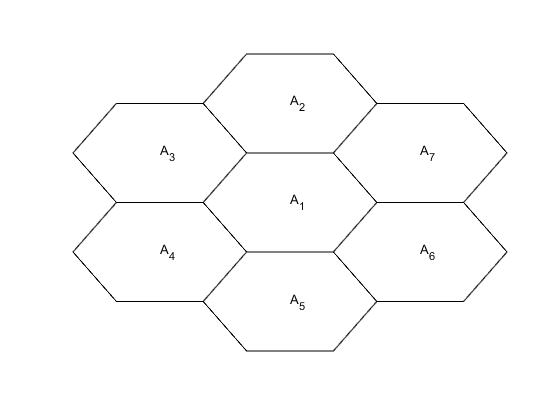
\includegraphics[width=4in]{latex/images/N1.jpg}}
\caption{Example of cell layout where N=1.}
\label{N1}
\end{figure}

\begin{figure}[h]
\centerline{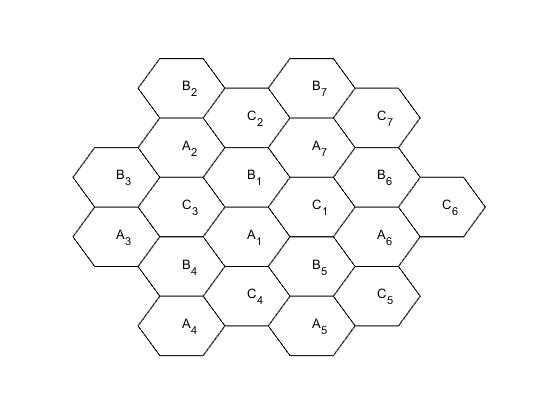
\includegraphics[width=4in]{latex/images/N3.jpg}}
\caption{Example of cell layout where N=3}
\label{N3}
\end{figure}

\begin{figure}[h]
\centerline{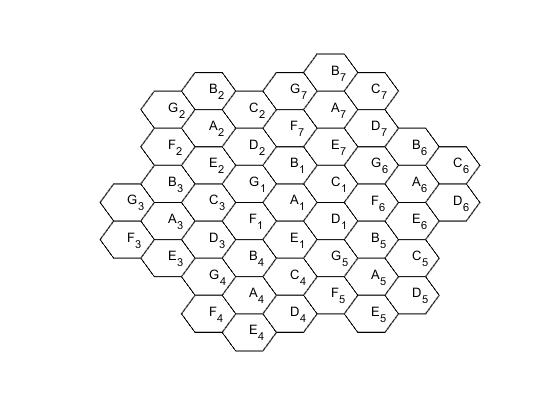
\includegraphics[width=4in]{latex/images/N7.jpg}}
\caption{Example of cell layout where N=7}
\label{N7}
\end{figure}
\clearpage
\section{How To Run}\label{run}

The code is straight forward to run. The demo is already set up to run and generate a movie called 'demo.avi' directly into the doc folder. At the top of the demo file there are parameters that can be edited to change the simulation.

Functions that were created and can be tested:
\begin{verbatim}


function [cell_names, cell_centers] = generateCluster(
		 center_position, iValue, jValue, cellRadius )
--This generates the cell_names and cell_centers
--to be used later in calculations and plotting

function success = drawCluster( cell_names, cell_positions, cell_radius )
--Draws the cluster that was generated.

function [cellNumber, tierNumber, center] = findServingCell(
			 mobileLocation, cellCenters, cellNames )
--This finds the closest serving cell near the mobile user. 
--Returns which cell is closest.

function power = friisFreeSpace(d)
--This calculates the power based off of the distance

function [r,g,b] = generateColor(Pr)
--This generates a color for the line and user based on the recieved power

\end{verbatim}

%\clearpage
%----------------------------------------------------------------------------------------
%	BIBLIOGRAPHY
%----------------------------------------------------------------------------------------

%\bibliography{bibliography/IEEEabrv,bibliography/bibliography}
%\bibliographystyle{ieeetr}
%\bibliographystyle{IEEEtran}
%\bibliography{sample}

%----------------------------------------------------------------------------------------

\end{document}
